\documentclass[10pt,conference,compsocconf]{IEEEtran}
% Computer Modern typewriter for code names (available in every LaTeX setup).
\renewcommand{\ttdefault}{cmtt}

\usepackage{hyperref}
\usepackage{graphicx}
\usepackage{amsmath}
\usepackage{booktabs}

\begin{document}

\title{Predicting Heart Disease from Survey Data:\\
Linear Models versus Boosted Trees in NumPy}

\author{
  Mehrdad Salehi, Reza Chehreghani, Brayan Kaelin\\
  \textit{School of Computer and Communication Sciences, EPFL, Switzerland}
}

\maketitle

\begin{abstract}
We predict if a person has coronary heart disease from 321 answers of the
2015 BRFSS survey, using only NumPy. The linear models from the course
underfit and stay below a validation F1 of 0.42. One-hot encoding improves
Ridge regression from 0.416 to 0.427, and our own gradient-boosted decision
trees reach 0.452 on validation and 0.454 on the AIcrowd test set. We also
show that the decision threshold matters a lot, and that one survey question
gives away the label for 2.7\% of the positive cases.
\end{abstract}

\section{Introduction}
For every person we predict if they have coronary heart disease (+1) or not
($-1$). We have 328{,}135 labelled and 109{,}379 test persons with 321
features: numbers, coded answers (e.g.\ 7 = ``don't know'') and many missing
values (147 features are missing for more than half of the persons). Only
8.83\% of the persons are positive, so we use the F1 score of the positive
class, $F_1 = 2PR/(P+R)$ with precision $P$ and recall $R$. Accuracy is not
useful here: always answering $-1$ gives 91.2\% accuracy but $F_1=0$.

\section{How we evaluate}
We split the labelled data per class into 80\% training and 20\% validation
(seed 42): 262{,}508 and 65{,}627 rows (5{,}795 positives). All models use
this split, and everything the preprocessing learns (categories, medians,
means, standard deviations, bin edges) comes from the training rows only.
Each model gives a score, and we predict +1 when the score is at least a
threshold $t$, chosen to maximize the validation F1 (grid with step 0.01).
Resampling the validation rows changes F1 by about 0.005, so we treat smaller
differences as ties. Because we also choose the hyperparameters on these
rows, our validation F1 is a bit optimistic. We used one hold-out split
instead of $k$-fold cross-validation because one tree model needs 5 to 15
minutes to train. As an independent check, we retrain the final models on all
labelled rows with the same settings and submit them to AIcrowd.

\section{Feature processing}
\textbf{Reviewed rules.} We checked some features in the CDC
codebook~\cite{brfss}. We remove \texttt{SEQNO} and \texttt{\_PSU} (the same
record number), set ``don't know'' and ``refused'' of \texttt{GENHLTH} (7, 9)
and \texttt{PHYSHLTH} (77, 99) to missing, set \texttt{PHYSHLTH} 88
(``none'') to 0 days, and add a missing indicator for both features.

\textbf{Missing values carry information.} Many answers are missing on
purpose, because some questions are only asked to some persons. For example,
\texttt{BPMEDS} (blood pressure medication) is only answered by the 40\% of
persons with high blood pressure: 16.3\% of them are positive, but only 3.8\%
of the others.

\textbf{Linear models.} We fill missing values with the training median. In
the one-hot version, each column with at most 10 different training values
(223 columns) is replaced by one 0/1 column per value seen in training plus
one for missing values (a new value gives zeros). Then we standardize all
columns and add a bias column (322 columns, or 1{,}283 with one-hot).
\textbf{Trees} use the raw values put into bins: one bin per value if a
feature has fewer than 64 values, otherwise 63 quantile bins, and one bin for
missing values.

\textbf{Label leakage.} \texttt{HAREHAB1} asks about rehabilitation after a
heart attack, so only persons who reported one (which is part of the label
definition) answer it: all 773 of them are positive (2.7\% of the positives).
It is also in the test data, so we kept it, but we report it here
(\texttt{STREHAB1}, after a stroke, is a weaker case with 36\% positives).

\section{Models}
\textbf{Required methods} (\texttt{implementations.py}). We implemented
linear regression with gradient descent and with SGD (one sample per step) on
$\mathcal{L}=\frac{1}{2N}\|y-Xw\|^2$, least squares and Ridge regression with
the normal equations $(X^\top X+2N\lambda I)w=X^\top y$, logistic regression
with gradient descent on $\frac{1}{N}\sum_n[\log(1+e^{x_n^\top w})-y_n x_n^\top
w]$ (with \texttt{logaddexp} for stability), and its regularized version with
$\lambda\|w\|^2$ (gradient term $2\lambda w$). All six pass the public grading
tests of the course. In our experiments we use logistic regression
($\gamma=0.01$, 5{,}000 steps, $w_0=0$, labels 0/1) and Ridge regression on
the labels $\pm1$ with $\lambda\in\{10^{-6},10^{-5},\dots,1\}$; with a small
$\lambda$, Ridge gives the least-squares solution that the two MSE methods
converge to. We did not tune the regularized logistic regression, because the
linear models already underfit and a larger $\lambda$ only made Ridge worse.

\textbf{Gradient-boosted trees} (\texttt{boosting.py}). Because the linear
models underfit, we implemented a non-linear model, following
XGBoost~\cite{xgboost,friedman}. A tree asks a few yes/no questions about the
features, and boosting adds many small trees, each one correcting the errors
of the previous ones. We start from the log-odds of the training positive
rate, and each tree is fitted to the gradient $g=p-y$ and Hessian $h=p(1-p)$
of the logistic loss. From the sums of $g$ and $h$ per node, feature and bin
we get, for every threshold (and both sides for missing values), the gain
$\frac{G_L^2}{H_L+\lambda}+\frac{G_R^2}{H_R+\lambda}-\frac{G^2}{H+\lambda}$,
and we keep the best split. A leaf predicts the Newton step $-G/(H+\lambda)$
with $\lambda=1$, and each child needs $H\ge1$. Trees grow level by level up
to depth $d$, each uses a random half of the training rows~\cite{stochastic}
and is added with learning rate $\eta$. We keep the number of trees with the
lowest validation logistic loss. We tested our split search against a
brute-force search.

\section{Results}
\begin{table}[t]
\caption{Validation F1 (best threshold) and AIcrowd test F1.}
\label{tab:models}
\centering
\small
\setlength{\tabcolsep}{4pt}
\begin{tabular}{@{}lcc@{}}
\toprule
Model & Val.\ F1 & Test F1 \\
\midrule
Always $-1$ (accuracy 0.912) & 0.000 & -- \\
Logistic regression, GD ($t=0.19$) & 0.418 & -- \\
Ridge, $\lambda=10^{-5}$ ($t=-0.58$) & 0.416 & -- \\
Ridge + one-hot, $\lambda=10^{-5}$ ($t=-0.60$) & 0.427 & 0.436 \\
Trees $d=1$, $\eta=0.1$, 400 trees & 0.444 & -- \\
Trees $d=3$, $\eta=0.1$, 331 trees ($t=0.21$) & 0.449 & 0.452 \\
Trees $d=5$, $\eta=0.1$, 224 trees & 0.444 & -- \\
\textbf{Trees $d=3$, $\eta=0.05$, 800 trees ($t=0.21$)} & \textbf{0.452} & \textbf{0.454} \\
\bottomrule
\end{tabular}
\end{table}

\begin{table}[t]
\caption{Ablations (validation F1).}
\label{tab:ablation}
\centering
\small
\begin{tabular}{@{}lc@{}}
\toprule
\multicolumn{2}{@{}l}{\emph{Ridge: feature processing}} \\
Original features & 0.414 \\
+ reviewed rules & 0.416 \\
+ one-hot (without rules) & 0.428 \\
+ reviewed rules + one-hot & 0.427 \\
\midrule
\multicolumn{2}{@{}l}{\emph{Ridge: regularization (reviewed)}} \\
$\lambda=10^{-5}$ / $10^{-2}$ / $1$ & 0.416 / 0.412 / 0.394 \\
\midrule
\multicolumn{2}{@{}l}{\emph{Trees: tuning}} \\
$d=3$, $\eta=0.1$ (331 trees) & 0.449 \\
$d=4$, $\eta=0.1$ (234 trees) & 0.446 \\
$d=3$, $\eta=0.05$ (798 trees) & 0.452 \\
$d=4$, $\eta=0.05$ (488 trees) & 0.450 \\
Average of 3 seeds ($d=4$, $\eta=0.05$) & 0.450 \\
Blend, Ridge weight 0 / 0.2 / 0.5 & 0.451 / 0.448 / 0.442 \\
\bottomrule
\end{tabular}
\end{table}

\begin{figure}[t]
\centering
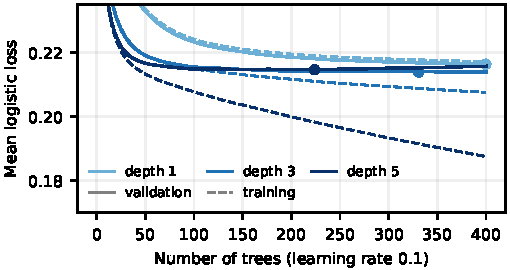
\includegraphics[width=\columnwidth]{figures/learning_curves.pdf}
\caption{Training (dashed) and validation (solid) logistic loss of the boosted
trees. Dots: lowest validation loss. Depth 1 underfits (both curves together),
depth 5 overfits (the validation loss goes up after 224 trees).}
\label{fig:curves}
\end{figure}

\begin{figure}[t]
\centering
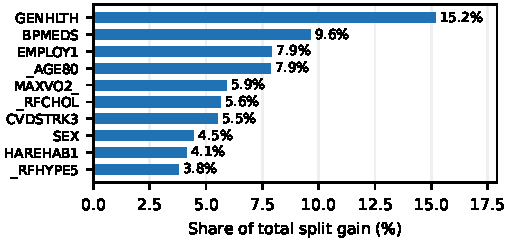
\includegraphics[width=\columnwidth]{figures/feature_importance.pdf}
\caption{Top 10 features of the $d=3$, $\eta=0.1$ trees by share of the total
split gain.}
\label{fig:importance}
\end{figure}

Table~\ref{tab:models} compares the models and Table~\ref{tab:ablation} shows
the effect of each change. Our final model (last row of
Table~\ref{tab:models}) has a validation precision of 0.376, recall of 0.567
and accuracy of 0.879.

\textbf{The linear models underfit.} The training and validation losses are
almost the same (logistic: 0.2282 and 0.2284; Ridge: 0.1358 and 0.1360), and
F1 only goes down when $\lambda$ grows.

\textbf{One-hot encoding} improves F1 by 0.011 to 0.014, because codes like
``don't know'' and missing values get their own weight instead of being used
as numbers. With one-hot, our hand-written rules do not matter anymore.

\textbf{The trees} improve F1 by 0.024 over Ridge with one-hot on validation
and by 0.018 on the test set. Depth 1 trees (one split each, so no
interactions) already give most of this gain, so the main benefit comes from
thresholds on single features and the missing bins. Depth 3 adds a little
(validation loss from 0.2164 to 0.2139), so some interactions help, while
depth 5 overfits (Fig.~\ref{fig:curves}). A smaller learning rate gives a
small gain. Averaging seeds or blending with Ridge does not help more than
the noise, so the trees already contain what Ridge learns.

\textbf{The threshold matters a lot.} With 8.8\% positives, few
probabilities are above 0.5. For the $d=3$, $\eta=0.1$ trees, F1 is 0.251 at
$t=0.5$ (precision 0.61, recall 0.16) but 0.449 at $t=0.21$.

\textbf{Important features.} The trees mostly use general health, blood
pressure medication, employment (retired or unable to work), age,
cholesterol, stroke and sex (Fig.~\ref{fig:importance}), all known risk
factors. The leaking \texttt{HAREHAB1} gives 4.1\% of the gain.

\section{Conclusion}
The linear models underfit these data. One-hot features help, but our
boosted trees help more (test F1 0.454), and the validation and test scores
agree (Table~\ref{tab:models}). \texttt{run.py} reproduces our best
submission in about 15 minutes (fixed seeds), and \texttt{train.py} and
\texttt{tune\_boosting.py} reproduce both tables.

\begin{thebibliography}{4}
\bibitem{xgboost} T.~Chen and C.~Guestrin, ``XGBoost: A scalable tree boosting
system,'' in \emph{Proc. ACM SIGKDD}, 2016, pp.~785--794.
\bibitem{friedman} J.~H. Friedman, ``Greedy function approximation: A gradient
boosting machine,'' \emph{Annals of Statistics}, vol.~29, no.~5,
pp.~1189--1232, 2001.
\bibitem{stochastic} J.~H. Friedman, ``Stochastic gradient boosting,''
\emph{Computational Statistics \& Data Analysis}, vol.~38, no.~4,
pp.~367--378, 2002.
\bibitem{brfss} Centers for Disease Control and Prevention, ``Behavioral Risk
Factor Surveillance System: 2015 codebook report,'' 2016.
\end{thebibliography}

\end{document}
